\documentclass[../ai_in_finance]{subfiles}
\usepackage[margin=1in]{geometry}
\usepackage{tikz}
\usetikzlibrary{positioning}
\usepackage{amsmath}
\usepackage{amssymb}
\usepackage{booktabs}
\usepackage{draftwatermark}
\usepackage{floatrow}

\SetWatermarkText{WSuo@Queensu.ca}
\SetWatermarkScale{1.4}
\SetWatermarkColor{gray!35}
\SetWatermarkAngle{45}

\usepackage{makeidx}
\makeindex

\begin{document}

\chapter{Time Series Analysis and Forecasting}

\section{Introduction}

Almost every dataset encountered so far in this book, prices in Chapter 2, financial statement line items in Chapter 4, credit spreads in Chapter 5, has an implicit time dimension: observations arrive in a sequence, and that sequence usually carries information that a model ignoring order would throw away.

This chapter makes time itself part of the model. It introduces the statistical vocabulary for describing dependence across time, stationarity, autocorrelation, and volatility clustering, and the classical models built on that vocabulary: autoregressive and moving-average models, ARIMA, GARCH, and state-space models.

Two worked examples run through the chapter: a short, hand-computable interest-rate-deviation series used to fit and forecast an autoregressive model, and the AssetA return series first introduced in Chapter 2, reused here to illustrate how GARCH captures volatility clustering. Beyond these two running examples, the chapter also introduces formal stationarity testing, seasonal models, and two ways of extending single-series analysis to several related series at once, cointegration\index{cointegration} and vector autoregression\index{vector autoregression (VAR)}.

Before closing, it returns to a promise made in Chapter 6: why cross-validation\index{cross-validation}, as normally practiced in machine learning, must be modified for time series data.

The chapter follows the same order an analyst would actually work through a new series: first establish whether it is stationary (Section~\ref{sec:adf-test}) and how strongly it depends on its own past (Section~\ref{sec:acf-section}), then fit and forecast a model on that basis (Section~\ref{sec:ar1-example}), quantifying the uncertainty around that forecast rather than reporting a single number (Section~\ref{sec:ci-pvalue}). The chapter then widens the lens from one series to several at once, cointegration (Section~\ref{sec:cointegration}) for pairs that move together, and the Kalman filter\index{Kalman filter} (Section~\ref{sec:kalman-example}) for a state that evolves and is only noisily observed, before closing with the walk-forward validation discipline that Chapters 8 and 11 both depend on directly.

Nearly every later chapter in this book that touches a time-ordered quantity, GARCH-based volatility in Chapter 8, momentum and mean-reversion trading signals in Chapter 11, cites this chapter's vocabulary rather than re-deriving it.

\section{Why Time Series Analysis Matters in Finance}\index{Why Time Series Analysis Matters in Finance}

Financial data are overwhelmingly time series: daily prices, quarterly earnings, monthly inflation, tick-by-tick trades. Three features of financial time series make them harder to work with than the typical machine learning dataset. First, observations are not independent; today's return is statistically related to yesterday's, even if only weakly, which violates the independent-and-identically-distributed assumption behind many standard statistical procedures. Second, the variance of returns is itself time-varying, quiet periods are followed by quiet periods and volatile periods by volatile periods, a phenomenon called volatility clustering.

Third, the underlying process generating the data can change over time (Chapter 6's non-stationarity concern), so a model fit on one period may not describe the next.

Time series methods exist precisely to handle these features rather than assume them away. They also underpin much of the rest of this book: the risk models in Chapter 8 need a volatility forecast, the portfolio methods in Chapter 10 need a covariance forecast, and the trading strategies in Chapter 11 need to know whether a signal is transient noise or a persistent pattern.

It is worth being explicit about what makes this chapter's models different from the regression and classification models of Chapter 6, even though both ultimately involve fitting parameters to minimize a loss function. A standard machine learning model assumes each training observation is drawn independently from the same underlying distribution as every other observation, which is precisely the assumption a time-ordered dataset violates: today's return is not independent of yesterday's, and a model that ignores this dependence, for example by randomly shuffling a time series before splitting it into training and test sets, will produce badly misleading performance estimates.

Every technique in this chapter, from the correlogram to GARCH to walk-forward validation, exists specifically to model, exploit, or correctly evaluate a model in the presence of this dependence, rather than assuming it away.

\section{Stationarity, White Noise, and Random Walks}\index{Stationarity, White Noise, and Random Walks}
\label{sec:random-walk}

Suppose an analyst fits a seemingly solid model relating an interest rate series to its own past values, only to find the fitted relationship falls apart the moment new data arrives, not because the estimation was done incorrectly, but because the series itself was never behaving consistently enough to model in the first place. This section makes precise exactly what kind of consistency a time series needs for a fitted model to have any hope of generalizing. A time series $\{X_t\}$ is weakly stationary if its mean and variance do not change over time and the covariance between $X_t$ and $X_{t-k}$ depends only on the lag $k$, not on $t$ itself:
\begin{equation*}
\mathbb{E}[X_t] = \mu, \qquad \text{Var}(X_t) = \sigma^2, \qquad \text{Cov}(X_t, X_{t-k}) = \gamma_k \text{ for all } t.
\end{equation*}
Stationarity matters because most time series models, including every model in this chapter, are built on the assumption that the statistical relationships estimated from the past will continue to hold; without it, there is no reason to expect a fitted model to generalize at all.

White noise is the simplest stationary process: a sequence $\varepsilon_t$ with mean zero, constant variance $\sigma^2$, and zero covariance at every nonzero lag, $\text{Cov}(\varepsilon_t, \varepsilon_{t-k}) = 0$ for $k \ne 0$. White noise is unpredictable by construction and serves as the building block, the ``noise,'' in every model that follows. 

A slightly stronger notion, strict stationarity, requires that the entire joint probability distribution of any collection of observations be unaffected by shifting them in time, not just their first two moments (mean and variance); weak stationarity, defined above, is what almost all of the practical models in this chapter actually rely on, since it is both easier to verify from data and sufficient for the estimation methods used throughout.

A random walk is $P_t = P_{t-1} + \varepsilon_t$, and it is not stationary: its variance grows with $t$ (specifically $\text{Var}(P_t) = t\sigma^2$ if $P_0$ is fixed), so its statistical behavior genuinely changes over time.

Asset prices behave approximately like random walks, which is exactly why Chapter 2 worked with returns, $R_t = (P_t - P_{t-1})/P_{t-1}$, rather than price levels: returns are much closer to stationary, since they do not inherit the ever-growing variance of the price level. This is not a minor technical preference; fitting a stationary-series model such as AR or ARMA directly to a non-stationary price level produces meaningless, unstable estimates, which is why the first step in almost any time series analysis is to check whether the series needs to be differenced (transformed to $\Delta X_t = X_t - X_{t-1}$) or converted to returns before modeling.

\section{Testing for Stationarity: The Augmented Dickey-Fuller Test}\index{Testing for Stationarity: The Augmented Dickey-Fuller Test}
\label{sec:adf-test}

Deciding whether a series is stationary should not rest on visual inspection alone; the standard formal test is the (augmented) Dickey-Fuller test\index{Dickey-Fuller Test}. The test rewrites the AR(1) model 
$$X_t = c + \phi X_{t-1} + \varepsilon_t$$ 
in first-difference form,
\begin{equation*}
\Delta X_t = \alpha + \gamma X_{t-1} + \varepsilon_t, \qquad \gamma = \phi - 1,
\end{equation*}
and tests the null hypothesis $H_0: \gamma = 0$ (equivalent to $\phi = 1$, a unit root, meaning the series is a non-stationary random walk) against the alternative $H_1: \gamma < 0$ (meaning $\phi < 1$, so the series is stationary and mean-reverting). The ``augmented'' version adds lagged difference terms 
$$\Delta X_{t-1}, \Delta X_{t-2}, \ldots$$ 
to the right-hand side to account for additional autocorrelation, but the core logic, testing whether $\gamma$ is significantly negative, is unchanged.

Applying the (non-augmented) test to the interest-rate deviation series in Table~\ref{tab:ar1_data} means regressing $\Delta X_t$ on $X_{t-1}$:
\begin{equation*}
\hat\gamma = -0.290, \qquad SE(\hat\gamma) = 0.259, \qquad t\text{-statistic} = \frac{\hat\gamma}{SE(\hat\gamma)} \approx -1.12.
\end{equation*}
Notice that $\hat\gamma = -0.290$ is consistent with the AR(1) coefficient fitted earlier, since 
$$\hat\phi - 1 = 0.710 - 1 = -0.290$$ 
exactly. Critically, the Dickey-Fuller test does not use standard normal or $t$-distribution critical values, because under the null hypothesis of a unit root the test statistic has a nonstandard distribution; the relevant critical value at the 5\% level (with a constant term and no trend) is approximately $-2.89$, not the familiar $-1.96$. 

Since $|-1.12| < 2.89$, this test fails to reject the null hypothesis of a unit root, even though the AR(1) coefficient of 0.71 and the visibly decaying correlogram both suggest genuine mean reversion. This apparent contradiction is not a flaw in the test; it is a direct consequence of the sample size: with only 8 observations, the Dickey-Fuller test has very little statistical power to distinguish a stationary process from a unit-root process, exactly the ``limited effective sample size'' challenge flagged later in this chapter. In practice, the ADF test is typically applied to series with many more observations than this illustrative example, where its power to detect stationarity is much greater.

\section{Autocorrelation and the Correlogram}\index{Autocorrelation and the Correlogram}
\label{sec:acf-section}

Suppose an analyst has just concluded, from the ADF test above, that an interest-rate series is likely mean-reverting rather than a random walk, and now wants to know exactly how far back its memory extends: does today's value mainly reflect yesterday's, or does a shock from several periods ago still leave a detectable trace? The autocorrelation function (ACF) answers this directly by measuring how strongly a series is related to its own past values. At lag $k$, it is defined as
\begin{equation*}
\rho_k = \frac{\gamma_k}{\gamma_0} = \frac{\text{Cov}(X_t, X_{t-k})}{\text{Var}(X_t)},
\end{equation*}
and is estimated from a sample of $T$ observations with mean $\bar X$ as
\begin{equation*}
\hat\rho_k = \frac{\sum_{t=k+1}^{T} (X_t - \bar X)(X_{t-k} - \bar X)}{\sum_{t=1}^{T} (X_t - \bar X)^2}.
\end{equation*}
A plot of $\hat\rho_k$ against $k$ is called a correlogram, and it is one of the most commonly used diagnostic tools in time series analysis: white noise has a correlogram that is statistically indistinguishable from zero at every lag, while a genuinely autocorrelated series shows a clear pattern, decaying gradually for an autoregressive process, cutting off sharply for a pure moving-average process. Figure~\ref{fig:acf} shows the correlogram computed from the worked example in the next section.

Because $\hat\rho_k$ is estimated from a finite sample, it is subject to sampling error, and a common rule of thumb treats $\hat\rho_k$ as statistically indistinguishable from zero if it falls within an approximate 95\% confidence band of $\pm 1.96/\sqrt{T}$, where $T$ is the number of observations used to compute the ACF. For the 8-observation series analyzed in the next section, this band is $\pm 1.96/\sqrt{8} \approx \pm 0.693$, which is larger in magnitude than the sample autocorrelation $\hat\rho_1 = 0.497$ computed there; Figure~\ref{fig:acf} plots this band directly alongside the correlogram.

In other words, even the largest, most visually striking autocorrelation in this chapter's own worked example is not, strictly speaking, statistically distinguishable from zero at conventional confidence levels, purely because the sample is so small. This is not a contradiction of the chapter's earlier claim that the correlogram shows a clear AR(1) pattern; rather, it is a reminder, consistent with the ADF test's failure to reject a unit root in Section~\ref{sec:adf-test}, that with only 8 observations essentially no time series diagnostic can be fully trusted, and that the qualitative pattern (geometric decay) is more informative here than any individual significance test.

\section{A Worked Example: Fitting and Forecasting an AR(1) Model}\index{Fitting and Forecasting an AR(1) Model}
\label{sec:ar1-example}

This section works through the full lifecycle of a small time series model: fitting it to data, checking that its correlogram behaves as theory predicts, and using it to produce both a point forecast and, later in the chapter, a sense of how that forecast's uncertainty grows with the horizon. An autoregressive model of order 1, AR(1), expresses the current value as a linear function of the immediately preceding value plus noise:
\begin{equation*}
X_t = c + \phi X_{t-1} + \varepsilon_t, \qquad \varepsilon_t \sim \text{white noise}(0, \sigma^2).
\end{equation*}
The process is stationary if and only if $|\phi| < 1$, in which case its theoretical autocorrelation decays geometrically, $\rho_k = \phi^k$, and its long-run (unconditional) mean is $c/(1-\phi)$.

Table~\ref{tab:ar1_data} shows eight monthly observations of a short-term interest-rate deviation from its policy target, measured in basis points.

\begin{table}[htbp]
\centering
\caption{A short interest-rate deviation series (basis points)}
\label{tab:ar1_data}
\begin{tabular}{lrrrrrrrr}
\toprule
Month $t$ & 1 & 2 & 3 & 4 & 5 & 6 & 7 & 8 \\
Deviation $X_t$ & 9.0 & 8.0 & 7.0 & 7.0 & 5.0 & 6.0 & 4.0 & 4.0 \\
\bottomrule
\end{tabular}
\end{table}

The sample autocorrelations, computed directly from the formula above using the full-sample mean $\bar X = 6.25$, are $\hat\rho_1 = 0.50$, $\hat\rho_2 = 0.24$, and $\hat\rho_3 = 0.03$, plotted in Figure~\ref{fig:acf}. The roughly geometric decay, each lag's autocorrelation is a bit less than half the previous one, is exactly the signature an AR(1) process should produce.

\begin{figure}[htbp]
\centering
\begin{lrbox}{\bookmeasuredbox}
    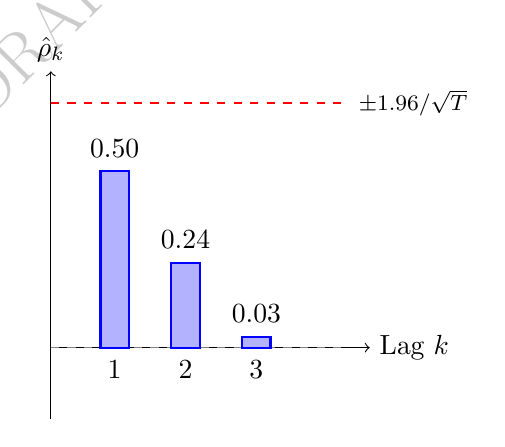
\begin{tikzpicture}[scale=0.9]
        \draw[->] (0,-1.0) -- (0,3.9) node[above] {$\hat\rho_k$};
        \draw[red,dashed,thick] (0,3.45) -- (4.2,3.45) node[right,black,font=\footnotesize] {$\pm 1.96/\sqrt{T}$};
        \draw[->] (0,0) -- (4.5,0) node[right] {Lag $k$};
        \draw[gray,dashed] (0,0) -- (4.2,0);
        \draw[thick,blue,fill=blue!30] (0.7,0) rectangle (1.1,2.49);
        \draw[thick,blue,fill=blue!30] (1.7,0) rectangle (2.1,1.20);
        \draw[thick,blue,fill=blue!30] (2.7,0) rectangle (3.1,0.15);
        \node[below] at (0.9,-0.05) {1};
        \node[below] at (1.9,-0.05) {2};
        \node[below] at (2.9,-0.05) {3};
        \node[above] at (0.9,2.55) {0.50};
        \node[above] at (1.9,1.26) {0.24};
        \node[above] at (2.9,0.21) {0.03};
    \end{tikzpicture}
\end{lrbox}
\ifdim\wd\bookmeasuredbox<0.65\linewidth
\setlength{\bookcapwidth}{0.65\linewidth}
\else
\setlength{\bookcapwidth}{\wd\bookmeasuredbox}
\fi
\ffigbox[\bookcapwidth]{
\usebox{\bookmeasuredbox}
}{
    \caption{Sample correlogram for the interest-rate deviation series in Table~\ref{tab:ar1_data}, with the approximate $95\%$ significance band $\pm 1.96/\sqrt{T}$ (dashed red; symmetric about zero, so only its positive side is drawn).}
    \label{fig:acf}
}
\end{figure}

The AR(1) coefficients are estimated the same way any linear regression is estimated, by regressing $X_t$ on $X_{t-1}$ using the OLS formulas from Chapter 6:
\begin{equation*}
\hat\phi = \frac{\sum_t (X_{t-1}-\bar X_{\text{lag}})(X_t - \bar X_{\text{cur}})}{\sum_t (X_{t-1}-\bar X_{\text{lag}})^2}, \qquad \hat c = \bar X_{\text{cur}} - \hat\phi\, \bar X_{\text{lag}},
\end{equation*}
where $\bar X_{\text{lag}}$ and $\bar X_{\text{cur}}$ are the means of the lagged and current values, respectively (each computed over the 7 available pairs, so they differ slightly from the full-sample mean $\bar X = 6.25$ used for the correlogram). Fitting this to Table~\ref{tab:ar1_data} gives
\begin{equation*}
\hat\phi = 0.71, \qquad \hat c = 1.19, \qquad R^2 = 0.60.
\end{equation*}
Since $|\hat\phi| = 0.71 < 1$, the fitted process is stationary, with an implied long-run mean of $\hat c/(1-\hat\phi) = 1.19/0.29 \approx 4.11$ basis points. Notice that this is noticeably different from the raw sample mean of 6.25: with only 8 observations, the AR(1) coefficient estimate carries substantial small-sample uncertainty, and the model-implied long-run mean should be treated as no more precise than the data that produced it. The one-step-ahead forecast, given the final observation $X_8 = 4.0$, is
\begin{equation*}
\hat X_9 = \hat c + \hat\phi\, X_8 = 1.19 + 0.71(4.0) \approx 4.03 \text{ basis points}.
\end{equation*}
This is the essential logic of every autoregressive forecast: today's fitted relationship, applied to the most recent observation, produces tomorrow's point forecast.

\subsection{Confidence Intervals and P-Values for Model Parameters}\index{Confidence Intervals and P-Values for Model Parameters}
\label{sec:ci-pvalue}

A point estimate such as $\hat\phi = 0.71$ is only half the story; without some sense of how precisely $\hat\phi$ is known, it is impossible to say whether the fitted mean reversion is a genuine feature of the process or an artifact of a short, noisy sample. 

Chapter 6's Section 6.4 built the standard-error, $t$-statistic, $p$-value, and confidence-interval machinery for exactly this purpose, including the correct (and the common incorrect) ways to state what a confidence interval means; that machinery applies here unchanged, since $\hat\phi$ is itself just an OLS slope, of $X_t$ on $X_{t-1}$, so this section applies the method rather than re-deriving it. For the AR(1) regression fitted above, with $n=7$ usable pairs and $2$ estimated parameters (so $n-2=5$ residual degrees of freedom),
\begin{equation*}
SE(\hat\phi) = \sqrt{\frac{\hat\sigma^2}{\sum_t (X_{t-1}-\bar X_{\text{lag}})^2}} \approx 0.259, \qquad \hat\sigma^2 = \frac{\text{SSR}}{n-2} \approx 1.187, \qquad t = \frac{\hat\phi}{SE(\hat\phi)} = \frac{0.71}{0.259} \approx 2.74,
\end{equation*}
where SSR is the sum of squared residuals from the fitted line. Under the null hypothesis $H_0: \phi = 0$ (no mean reversion at all, this month's deviation carries no information about next month's), this $t$-statistic follows a $t$-distribution with $5$ degrees of freedom and gives $p \approx 0.041$: by the conventional $5\%$ threshold, $\hat\phi = 0.71$ is (barely) significant, so the data offer modest evidence of genuine mean reversion, but the margin is thin. The corresponding $95\%$ confidence interval,
\begin{equation*}
\hat\phi \pm t^*_{0.975,\,5}\cdot SE(\hat\phi) = 0.71 \pm (2.571)(0.259) \approx (0.04,\ 1.38),
\end{equation*}
is wide, spanning nearly the entire plausible range from very weak to very strong mean reversion, and includes values close to $1$ (the unit-root boundary).

This is the same small-sample fragility flagged when the Dickey-Fuller test in Section~\ref{sec:adf-test} failed to reject a unit root despite $\hat\phi = 0.71$ visually suggesting real mean reversion: a $t$-statistic, a $p$-value, and a confidence interval are three views of the same underlying estimation uncertainty, and with only $8$ observations, that uncertainty is simply large. Applying the identical method to the intercept gives $SE(\hat c) \approx 1.750$, $t \approx 0.68$, and $p \approx 0.526$, so the intercept is not statistically distinguishable from zero at conventional significance levels, a much weaker result than the slope's.

Chapter 6's Section 6.4 already flagged the two practical warnings that apply here without modification: statistical significance is not the same as economic or financial significance, and testing many coefficients or candidate models against the same data inflates the chance that at least one spuriously crosses the $5\%$ threshold by pure luck.

That second warning is exactly the multiple-testing problem Section~\ref{sec:cointegration}'s discussion of pairs selection revisits concretely, fulfilling the forward pointer Chapter 6 itself made to this section: a single $p$-value below $0.05$ is far less persuasive when it is the best of twenty candidate pairs tried rather than the only pair considered.

\section{Multi-Step Forecasting and the Growth of Uncertainty}\index{Multi-Step Forecasting and the Growth of Uncertainty}

The one-step-ahead forecast above answers ``what happens next period,'' but many financial decisions require forecasting several periods ahead. For an AR(1) model, this is done recursively: use the one-step forecast $\hat X_9$ as if it were the actual next observation to produce $\hat X_{10} = \hat c + \hat\phi \hat X_9$, and continue in the same way for as many steps as needed. Applying this to the fitted model ($\hat\phi=0.71$, $\hat c=1.19$) starting from $X_8=4.0$ gives the forecasts in Table~\ref{tab:multistep}.

\begin{table}[htbp]
\centering
\caption{Multi-step-ahead AR(1) forecasts from month 8}
\label{tab:multistep}
\begin{tabular}{lrrrrr}
\toprule
Horizon $h$ & 1 & 2 & 3 & 5 & 10 \\
Forecast $\hat X_{8+h}$ & 4.03 & 4.06 & 4.07 & 4.09 & 4.11 \\
\bottomrule
\end{tabular}
\end{table}

Two features of Table~\ref{tab:multistep} illustrate general properties of stationary autoregressive forecasts. First, the forecasts converge smoothly toward the model's long-run mean of $\hat c/(1-\hat\phi) \approx 4.11$ as the horizon grows, rather than continuing to track short-run fluctuations; a stationary model's best guess about the distant future is essentially just its unconditional mean, since any information in today's observation about deviations from that mean fades geometrically at rate $\hat\phi$ per period.

Second, the uncertainty around these forecasts also grows with the horizon but, unlike a random walk, does not grow without bound: the variance of the $h$-step forecast is proportional to $\sum_{j=0}^{h-1} \hat\phi^{2j}$, which converges to $1/(1-\hat\phi^2) \approx 2.01$ times the one-step forecast variance as $h \to \infty$, rather than growing linearly with $h$ as it would for a non-stationary series. This is a direct, quantitative version of the qualitative warning in this chapter's challenges section that longer-horizon forecasts are less reliable than one-step forecasts, and it shows precisely how much less reliable, and why that unreliability eventually levels off, for a genuinely mean-reverting series.

\subsection{Diagnosing the Fit: The Ljung-Box Test and Choosing Between AR(1) and AR(2)}\index{Ljung-Box test}
\label{sec:ljung-box}

Fitting a model is not the end of the process; the residuals should be checked for leftover structure the model failed to capture, exactly the ``did this actually work'' question the Box-Jenkins methodology introduced later in this chapter is built around. The Ljung-Box test formalizes this check: it tests the joint null hypothesis that the first $h$ residual autocorrelations are all zero, meaning an adequately specified model should leave behind nothing but white noise, using the statistic
\begin{equation*}
Q = n(n+2)\sum_{k=1}^h \frac{\hat\rho_k^2}{n-k},
\end{equation*}
where $\hat\rho_k$ is the residuals' own sample autocorrelation at lag $k$ (computed exactly as in Section~\ref{sec:acf-section}, but applied to the residuals rather than the raw series) and $n$ is the number of residuals. Under the null hypothesis of a correctly specified model, $Q$ follows a chi-squared distribution with $h-p-q$ degrees of freedom, where $p$ and $q$ are the number of AR and MA parameters already estimated, subtracted because fitting those parameters already accounts for some of the dependence the test would otherwise attribute to unmodeled autocorrelation.

Applying this to the AR(1) model fitted above ($\hat\phi=0.71$, $\hat c=1.19$), the seven residuals are $(0.42, 0.13, 0.84,$ $-1.16, 1.26, -1.45, -0.03)$, giving residual autocorrelations $\hat\rho_1 = -0.68$ and $\hat\rho_2 = 0.49$, both considerably larger in magnitude than a well-fitting model's residuals should show. With $h=2$ lags and $p=1$ AR parameter, $Q = 7.91$ against a chi-squared distribution with $2-1=1$ degree of freedom, giving $p \approx 0.005$, comfortably below the conventional 5\% threshold.

The AR(1) model's residuals, in other words, are not well described as white noise: some genuine structure remains unmodeled.

This motivates asking whether a higher-order model captures more of that structure. Fitting an AR(2) model,
$$X_t = c + \phi_1 X_{t-1} + \phi_2 X_{t-2} + \varepsilon_t,$$
to the same six usable observations ($t=3,\ldots,8$; the sample must shrink by one further observation to accommodate the second lag, and the AR(1) model is refit on this identical six-observation sample so the two models' fit statistics are directly comparable) gives $\hat\phi_1 = 0.03$, $\hat\phi_2 = 0.88$, and a residual sum of squares of only $1.39$, versus $5.60$ for the AR(1) model refit on the same six observations, a dramatic improvement. Comparing the two models with the information criteria introduced in the ARIMA section below,
\begin{equation*}
\text{AIC} = n\ln(\text{SSR}/n) + 2k, \qquad \text{BIC} = n\ln(\text{SSR}/n) + k\ln n,
\end{equation*}
with $n=6$ throughout ($k=2$ and $k=3$ parameters for AR(1) and AR(2), respectively), gives
\begin{align*}
\text{AIC}_{\text{AR(1)}} &= 3.59, & \text{AIC}_{\text{AR(2)}} &= -2.76, \\
\text{BIC}_{\text{AR(1)}} &= 3.17, & \text{BIC}_{\text{AR(2)}} &= -3.39:
\end{align*}
both criteria favor AR(2) by a wide margin, even after the extra parameter's complexity penalty.

Yet this conclusion should be read with real caution rather than taken as a settled upgrade: an AR(2) model on only six observations is already using half of the sample's data points as estimated parameters ($k=3$ against $n=6$), precisely the ``limited effective sample size'' and ``model selection versus overfitting'' concerns raised later in this chapter's challenges section, so a dramatically lower AIC/BIC here is at least as likely to reflect a small sample's capacity to fit its own noise as it is a genuinely better-specified model. In a longer series, this same Ljung-Box-then-AIC/BIC workflow, fit a candidate model, test whether its residuals are white noise, and if not, compare a higher-order alternative using an information criterion, remains standard practice; it is only the tiny sample size here that makes the specific numerical conclusion (prefer AR(2)) less trustworthy than the procedure itself.

\section{Moving Averages and Exponential Smoothing}\index{Moving Averages and Exponential Smoothing}

Before turning to ARIMA and GARCH, it is worth introducing two much simpler forecasting tools that remain widely used because of their transparency. A simple moving average forecast uses the average of the most recent $m$ observations as the forecast for the next period,
\begin{equation*}
\hat X_{t+1} = \frac{1}{m}\sum_{i=0}^{m-1} X_{t-i}.
\end{equation*}
It is easy to compute and understand, but it weights all $m$ past observations equally and drops old observations abruptly once they fall outside the window.

Exponential smoothing addresses both issues by weighting all past observations, but with exponentially decaying weight on older data:
\begin{equation*}
\hat X_{t+1} = \alpha X_t + (1-\alpha)\hat X_t, \qquad 0 < \alpha < 1,
\end{equation*}
which can be expanded to show that $\hat X_{t+1}$ is a weighted average of every past observation, with weight $\alpha(1-\alpha)^i$ on the observation $i$ periods back.

A larger $\alpha$ makes the forecast react quickly to new information at the cost of more noise; a smaller $\alpha$ produces a smoother but slower-reacting forecast. Applied to Table~\ref{tab:ar1_data} with $\alpha = 0.4$ and an initial forecast $\hat X_1 = X_1 = 9.0$, the recursion produces a smoothed forecast that tracks the series' gradual decline without reacting sharply to any single observation, in contrast to the AR(1) model, which explicitly ties the forecast to the estimated mean-reversion coefficient $\hat\phi$ rather than only to recent history.

Simple exponential smoothing has an important limitation: because it forecasts using only a smoothed level, it always predicts a flat, unchanging line into the future, which performs poorly for a series with a clear trend, exactly the kind of gradual decline visible in Table~\ref{tab:ar1_data}. Holt's linear trend method\index{Holt's Linear Trend Method} addresses this by smoothing two components separately, a level $L_t$ and a trend $T_t$:
\begin{align*}
L_t &= \alpha X_t + (1-\alpha)(L_{t-1} + T_{t-1}), \\
T_t &= \beta (L_t - L_{t-1}) + (1-\beta) T_{t-1},
\end{align*}
and forecasts $h$ steps ahead as $\hat X_{t+h} = L_t + h T_t$, explicitly projecting the estimated trend forward rather than assuming it disappears. Applying this to Table~\ref{tab:ar1_data} with $\alpha=0.4$, $\beta=0.3$, an initial level $L_1=9.0$, and an initial trend $T_1 = X_2 - X_1 = -1.0$, the recursion produces a final level of $L_8 \approx 3.45$ and trend of $T_8 \approx -0.82$, giving a one-step-ahead forecast of
\begin{equation*}
\hat X_9 = L_8 + T_8 \approx 3.45 - 0.82 \approx 2.64.
\end{equation*}
This is noticeably lower than both the simple exponential smoothing forecast (about 4.50, computed above) and the AR(1) forecast (4.03, computed in Section~\ref{sec:ar1-example}), because Holt's method explicitly extrapolates the series' downward trend rather than assuming the series will revert toward a stable mean, as the AR(1) model does, or stay flat, as simple exponential smoothing does.

Which forecast is more appropriate depends entirely on whether the analyst believes the series is genuinely trending or is instead a mean-reverting process passing through a temporarily low patch, a judgment call that no single mechanical formula can resolve and that connects directly back to the stationarity testing in Section~\ref{sec:adf-test}: a trending (non-stationary) series is better suited to Holt's method, while a mean-reverting (stationary) series is better suited to the AR(1) approach. A further extension, Holt-Winters smoothing, adds a third seasonal component to handle the kind of periodic patterns discussed in the SARIMA section below.

\section{ARIMA Models}\index{ARIMA Models}

Suppose a shock, a one-time data-reporting glitch, say, appears to influence a series for exactly one additional period before vanishing completely, rather than decaying away gradually forever the way the AR(1) model above implies. The AR(1) model in Section~\ref{sec:ar1-example} is a special case of a much broader family built to capture exactly this kind of finite-memory dependence, among others. A moving-average model of order $q$, MA($q$), expresses the current value as a function of recent noise terms rather than recent levels,
\begin{equation*}
X_t = \mu + \varepsilon_t + \theta_1 \varepsilon_{t-1} + \cdots + \theta_q \varepsilon_{t-q},
\end{equation*}
and combining autoregressive and moving-average terms gives an ARMA($p,q$) model. Because many financial series (prices, but also many macroeconomic series) 
are non-stationary in levels 
but stationary after differencing, the ARIMA($p,d,q$) model applies an ARMA($p,q$) model to the series after 
differencing $d$ times: $d=1$ removes a linear trend, $d=2$ removes a quadratic trend, and so on. In practice, $d$ is rarely more than 1 or 2 for financial data, 
since returns (a $d=1$ difference of log prices) are already close to stationary.

The MA($q$) component has a theoretical autocorrelation structure that is the mirror image of the AR($p$) process introduced earlier in this chapter, and this 
contrast is precisely what makes the ACF and PACF useful diagnostic tools together. For an MA(1) process $X_t = \mu + \varepsilon_t + \theta \varepsilon_{t-1}$, 
the theoretical autocorrelation is $\rho_1 = \theta/(1+\theta^2)$ and $\rho_k=0$ for every lag $k>1$; for $\theta=0.6$, this gives $\rho_1 = 0.6/1.36 \approx 0.441$ and 
then an abrupt drop to zero at lag 2, in sharp contrast to the AR(1) correlogram in Figure~\ref{fig:acf}, whose autocorrelations decay gradually across every lag 
rather than cutting off sharply. This is the basis of the Box-Jenkins identification rule: a correlogram (ACF) that cuts off sharply after lag $q$ suggests an 
MA($q$) model, while a partial autocorrelation function that cuts off sharply after lag $p$ suggests an AR($p$) model; a series where both decay gradually 
suggests a mixed ARMA($p,q$) model, for which the specific orders are typically chosen by comparing information criteria across a small number of candidates
 rather than by reading the correlogram alone.

Choosing the orders $p$, $d$, and $q$ is traditionally done with the Box-Jenkins methodology\index{Box-Jenkins Methodology}: examine the ACF and its partial-autocorrelation 
counterpart (the PACF\index{Partial Autocorrelation Function (PACF)}, which measures the correlation between $X_t$ and $X_{t-k}$ after removing the influence of the 
intervening lags) to identify candidate orders, fit several candidate models, and compare them using an information criterion such as AIC or BIC, which penalize 
model complexity to avoid simply picking the model with the most parameters. This is the time series analogue of the model-selection problem in Chapter 6: 
more lags will always fit the training data at least as well, but a model with too many lags overfits sample noise exactly as a high-degree polynomial does.

Many financial and economic series also exhibit seasonality, a repeating pattern at a fixed period, such as retail sales spiking every December or trading 
volume dipping every summer. SARIMA (Seasonal ARIMA)\index{SARIMA (Seasonal ARIMA)} extends ARIMA by adding a second set of autoregressive, differencing, and 
moving-average terms operating at the seasonal period $s$, denoted $\text{SARIMA}(p,d,q)(P,D,Q)_s$: the non-seasonal part $(p,d,q)$ captures short-run 
dynamics exactly as before, while the seasonal part $(P,D,Q)_s$ captures dependence at lags $s, 2s, 3s, \ldots$. For example, a monthly retail sales 
series might be modeled as $\text{SARIMA}(1,1,1)(1,1,1)_{12}$, where the seasonal terms specifically model the relationship between each month and 
the same month one year ($s=12$ months) earlier, on top of the ordinary month-to-month dynamics the non-seasonal terms capture. 

Seasonal differencing, $\Delta_s X_t = X_t - X_{t-s}$, is the seasonal analogue of the ordinary differencing introduced above, and it is applied when a series 
exhibits a seasonal unit root, an extension of the stationarity testing in Section~\ref{sec:adf-test} to the seasonal frequency. Most asset return series in 
finance show little seasonality at the daily frequency, which is why the GARCH and ARIMA examples elsewhere in this chapter do not require a seasonal extension, 
but seasonality is common and important in macroeconomic series (retail sales, employment, seasonally-adjusted GDP) that feed into the fundamental analysis of
 Chapter 4 and the macroeconomic risk factors of Chapters 8 and 9.

\section{Cointegration and Pairs Trading}\index{Cointegration and Pairs Trading}
\label{sec:cointegration}

Section~\ref{sec:adf-test} showed that individual price series are typically non-stationary. A remarkable exception arises when two non-stationary series move together closely enough that a specific linear combination of them is stationary, a relationship called cointegration. Two stocks in the same industry, for example, might each individually wander like a random walk, yet the spread between their prices could still revert reliably to a stable long-run relationship, because both are driven by the same industry-wide fundamentals.

Table~\ref{tab:pairs_trading} shows six days of prices for two hypothetical bank stocks.

\begin{table}[htbp]
\centering
\caption{Prices for two hypothetical cointegrated bank stocks}
\label{tab:pairs_trading}
\begin{tabular}{lrrrrrr}
\toprule
Day & 1 & 2 & 3 & 4 & 5 & 6 \\
Stock A & 50 & 51 & 53 & 52 & 54 & 55 \\
Stock B & 48 & 49 & 50 & 50 & 51 & 52 \\
Spread ($A-B$) & 2 & 2 & 3 & 2 & 3 & 3 \\
\bottomrule
\end{tabular}
\end{table}

Both individual price series trend upward and would likely fail a stationarity test on their own, exactly like the random walk introduced earlier in this chapter. The spread, however, fluctuates narrowly around a mean of $\bar{s} = 2.5$ with a sample standard deviation of only $0.55$, far more stable than either underlying price series. The standard procedure for testing this formally, the Engle-Granger two-step method\index{Engle-Granger Two-Step Method}, first regresses one price on the other to estimate the cointegrating relationship,
\begin{equation*}
A_t = \alpha + \beta B_t + u_t,
\end{equation*}
which for this data gives $\hat\alpha = -12.5$ and $\hat\beta = 1.3$, and then applies the Dickey-Fuller test from Section~\ref{sec:adf-test} to the regression residuals $\hat u_t$: if the residuals reject the unit-root null (that is, they are stationary), the two series are cointegrated.

Note that this regression-based approach generalizes the simple $A_t - B_t$ spread used above (which implicitly assumes $\beta=1$) to an estimated hedge ratio $\hat\beta$, the number of shares of $B$ needed to offset one share of $A$; the simple difference is a reasonable approximation only when the two series move roughly one-for-one, which happens to be nearly true here since $\hat\beta=1.3$ is fairly close to 1.

This relationship is the foundation of pairs trading, a strategy covered in more depth in Chapter 11. In practice, the spread is standardized into a $z$-score, $z_t = (s_t - \bar s)/\hat\sigma_s$, so that trading rules can be stated in terms of standard deviations rather than the spread's raw units, which vary from one pair to the next. For the data in Table~\ref{tab:pairs_trading}, the final spread of 3 has a $z$-score of $z_6 = (3 - 2.5)/0.548 \approx 0.91$; a common rule of thumb opens a trade when $|z_t|$ exceeds roughly 2 (signaling an unusually wide or narrow spread) and closes it once $z_t$ reverts close to zero, so this particular spread, at just under one standard deviation from its mean, would not yet trigger a new trade under such a rule.

When the spread is unusually wide relative to its historical mean and standard deviation, a trader shorts the relatively expensive stock (here, $A$) and buys $\hat\beta$ shares of the relatively cheap one ($B$) for every share of $A$, betting that the spread will revert toward its mean; when the spread is unusually narrow, the trader takes the opposite position.

Because the strategy trades the spread rather than the direction of either stock, it is designed to profit regardless of whether the overall market rises or falls, a property called market neutrality, provided the cointegrating relationship itself remains stable, which is exactly the kind of assumption that can silently break down, a risk explored further when Chapter 11 discusses the practical risks of statistical arbitrage strategies.

\section{Vector Autoregression: Modeling Several Series Jointly}\index{Vector Autoregression: Modeling Several Series Jointly}

Every model so far in this chapter describes a single series in terms of its own past. A vector autoregression (VAR) extends the AR($p$) framework to several series simultaneously, allowing each variable to depend on its own past values and the past values of every other variable in the system. A VAR(1) model for two series $X_t$ and $Y_t$ is
\begin{align*}
X_t &= c_1 + a_{11} X_{t-1} + a_{12} Y_{t-1} + \varepsilon_{1,t}, \\
Y_t &= c_2 + a_{21} X_{t-1} + a_{22} Y_{t-1} + \varepsilon_{2,t},
\end{align*}
where the off-diagonal coefficients $a_{12}$ and $a_{21}$ capture cross-series dependence, for example how last month's interest rate might help predict this month's exchange rate, and vice versa. This is a natural way to model interconnected macroeconomic and financial series, such as interest rates, exchange rates, and inflation, together, rather than modeling each with a separate, univariate ARIMA model that ignores their interdependence.

A practically convenient feature of the VAR(1) system above is that, conditional on the lag order, each equation can be estimated separately by ordinary least squares, exactly the same OLS machinery introduced in Chapter 6, simply regressing $X_t$ on $X_{t-1}$ and $Y_{t-1}$, and separately regressing $Y_t$ on the same two lagged variables. Choosing the number of lags to include (extending the model to VAR($p$) for $p>1$) follows the same information-criterion logic, AIC or BIC, used to select ARIMA orders earlier in this chapter, since a VAR with too many lags relative to the amount of data will overfit just as readily as an over-parameterized univariate model.

VAR models are also the standard tool for testing Granger causality\index{Granger Causality}: variable $X$ is said to ``Granger-cause'' variable $Y$ if past values of $X$ improve the prediction of $Y$ beyond what past values of $Y$ alone provide, formally tested by checking whether the coefficients on lagged $X$ in the $Y$ equation (here, $a_{21}$) are statistically significant.

Granger causality is a statement about predictive usefulness, not causality in the deeper structural sense introduced in Chapter 1's discussion of correlation versus causation; a variable can Granger-cause another simply because it reflects the same information sooner, without one variable structurally driving the other at all.

Once a VAR is fitted, an impulse response function\index{Impulse Response Function} traces out how a one-time shock to one variable propagates through the system over subsequent periods: starting from the estimated coefficients, a hypothetical one-unit shock is applied to $\varepsilon_{1,t}$ (holding $\varepsilon_{2,t}=0$), and the model is iterated forward to see how both $X_{t+1}, X_{t+2}, \ldots$ and $Y_{t+1}, Y_{t+2}, \ldots$ respond over time, tracing the shock's full dynamic effect on both series rather than just its immediate, one-period impact.

This is a standard tool in macroeconomic policy analysis, for example tracing how a shock to short-term interest rates propagates to exchange rates and, eventually, inflation, and it is the multivariate analogue of the multi-step forecasting exercise carried out for the single-series AR(1) model earlier in this chapter. VAR models are widely used in macroeconomic forecasting and in studying how shocks propagate between markets, a natural multivariate extension of the single-series volatility and mean-reversion models developed throughout the rest of this chapter.

A concrete impulse response makes this propagation mechanism tangible. Suppose a VAR(1) has already been fitted (via the equation-by-equation OLS procedure above) to changes in a short-term interest rate $X_t$ and an exchange rate $Y_t$, with estimated coefficients $a_{11}=0.6$, $a_{12}=0.2$, $a_{21}=0.1$, and $a_{22}=0.7$ (intercepts omitted, since an impulse response tracks the deviation from baseline rather than the level). A one-unit shock to the interest rate at time $0$, with the exchange rate unshocked ($X_0=1$, $Y_0=0$), propagates as
\begin{equation*}
X_1 = 0.6(1) + 0.2(0) = 0.6, \qquad Y_1 = 0.1(1) + 0.7(0) = 0.1,
\end{equation*}
\begin{equation*}
X_2 = 0.6(0.6) + 0.2(0.1) = 0.38, \qquad Y_2 = 0.1(0.6) + 0.7(0.1) = 0.13,
\end{equation*}
and continuing this recursion gives
\begin{equation*}
X_3 = 0.254, \qquad Y_3 = 0.129, \qquad X_4 = 0.178, \qquad Y_4 = 0.116.
\end{equation*}
Two features of this impulse response are worth noting. First, even though the exchange rate was not shocked directly, it responds immediately, rising from $0$ to $0.1$ in a single period, purely through the cross-series coefficient $a_{21}=0.1$; this is exactly the kind of spillover a collection of separate, univariate ARIMA models, each blind to the other series, could never capture.

Second, the exchange rate's response does not simply fade monotonically alongside the interest rate's own decay: it initially rises further, from $0.1$ to $0.13$, before declining, because it continues to absorb the (still-elevated) interest rate for a second period even as the direct shock itself has already started to fade, a lagged-peak pattern that is a hallmark signature of genuine cross-series transmission rather than each series simply reverting independently.

Both series in this example do eventually decay back toward zero, which is not guaranteed by the individual coefficients alone; it depends on the stability of the whole coefficient matrix 
$$A = \begin{bmatrix} a_{11} & a_{12} \\ a_{21} & a_{22} \end{bmatrix}$$ 
jointly. The multivariate generalization of the univariate AR(1) stationarity condition $|\phi|<1$ is that every eigenvalue of $A$ must lie strictly inside the unit circle. For this system, $A$'s eigenvalues are exactly $0.5$ and $0.8$, both comfortably below $1$ in absolute value, confirming that the impulse response above must decay to zero eventually rather than explode, exactly as the numerical values $0.6, 0.38, 0.254, 0.178$ for $X$ and $0.1, 0.13, 0.129, 0.116$ for $Y$ already suggested.

A VAR fitted to real, non-stationary financial series (interest rate levels rather than changes, for example) can easily produce a coefficient matrix with an eigenvalue at or above 1, in which case the whole system is unstable and any impulse response or multi-step forecast built from it, however precisely computed, describes an explosive process rather than a meaningful economic dynamic. This is the direct multivariate analogue of the unit-root problem the Dickey-Fuller test in Section~\ref{sec:adf-test} is designed to detect in a single series, and it is exactly why a VAR, like an ARIMA model, is normally fit to differenced or otherwise stationary series rather than to raw levels.

\section{A Worked Example: PCA and Forecasting the Term Structure of Interest Rates}\index{PCA and Forecasting the Term Structure of Interest Rates}
\label{sec:pca-term-structure}

The VAR framework above handles two or three interconnected series comfortably, but Chapter 5's yield curve is not two series, it is a whole curve, one yield for every maturity a government issues debt at. Modeling eight or more maturities as a single high-dimensional VAR is possible in principle but wasteful in practice, because adjacent points on a yield curve are extremely highly correlated: the 2-year and 3-year yields, for instance, almost always move together.

Chapter 6 introduced principal component analysis (PCA)\index{Principal Component Analysis (PCA)} as the standard dimensionality-reduction method, finding the direction $w$ that maximizes $\text{Var}(Xw)$; applied to a panel of yield curve maturities rather than a panel of asset returns, PCA turns this redundancy into a genuine forecasting advantage, since a small number of extracted factors can carry nearly all of the curve's variation.

This worked example uses real data: the U.S. Treasury's daily par yield curve rates from January 2, 1990 through December 29, 2023, restricted to the eight maturities with essentially complete history over that period (3-month, 6-month, 1-year, 2-year, 3-year, 5-year, 7-year, and 10-year), giving $8{,}503$ daily observations. Applying PCA to this panel, mean-centered but not rescaled to unit variance (so that maturities with naturally larger yield swings are not artificially shrunk to match calmer ones), gives the explained variance ratios in Table~\ref{tab:pca_variance}.

\begin{table}[htbp]
\centering
\begin{lrbox}{\bookmeasuredbox}
\begin{tabular}{lrrrrr}
\toprule
Component & PC1 & PC2 & PC3 & PC4 & PC5 \\
\midrule
Variance explained & $95.95\%$ & $3.78\%$ & $0.22\%$ & $0.03\%$ & $0.01\%$ \\
\bottomrule
\end{tabular}
\end{lrbox}
\ifdim\wd\bookmeasuredbox<0.65\linewidth
\setlength{\bookcapwidth}{0.65\linewidth}
\else
\setlength{\bookcapwidth}{\wd\bookmeasuredbox}
\fi
\ttabbox[\bookcapwidth]{
\usebox{\bookmeasuredbox}
}{
\caption{Explained variance ratio by principal component, 1990--2023 Treasury yield curve panel}
\label{tab:pca_variance}
}
\end{table}

The first three components alone explain $99.96\%$ of the total variation across 34 years of daily yield curve moves, a striking result: an eight-dimensional forecasting problem collapses, with almost no loss of information, to a three-dimensional one. This is not a coincidence specific to this dataset; it is one of the most reproduced empirical results in fixed income, first documented by Litterman and Scheinkman (1991), and the three components have well-known, economically interpretable shapes once their loadings, the weight each maturity contributes to that component, are plotted against maturity.

\begin{figure}[htbp]
\centering
\begin{lrbox}{\bookmeasuredbox}
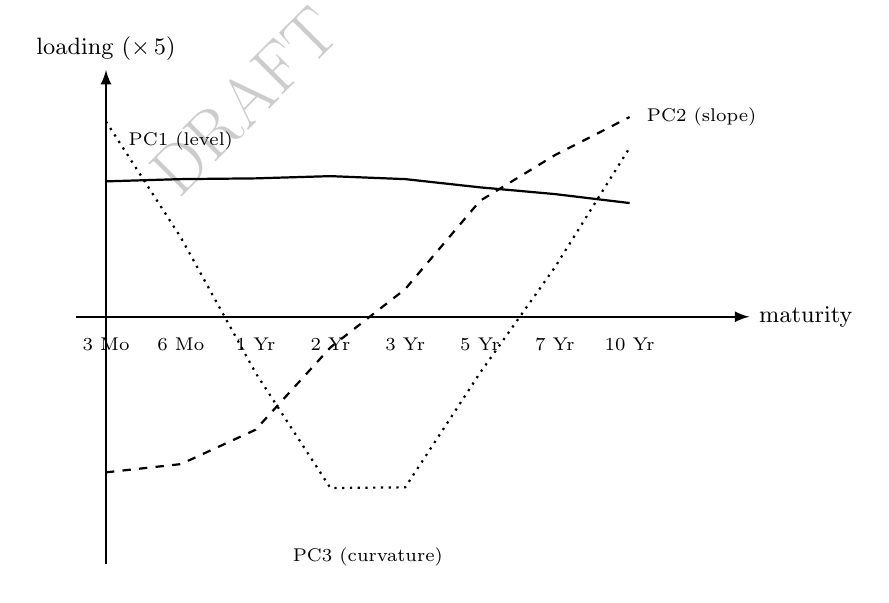
\begin{tikzpicture}[>=latex,thick,scale=0.95,transform shape]
\draw[->] (-0.4,0) -- (8.6,0) node[right,font=\small] {maturity};
\draw[->] (0,-3.3) -- (0,3.3) node[above,font=\small] {loading ($\times\,5$)};
\node[below,font=\scriptsize] at (0,-0.15) {3 Mo};
\node[below,font=\scriptsize] at (1,-0.15) {6 Mo};
\node[below,font=\scriptsize] at (2,-0.15) {1 Yr};
\node[below,font=\scriptsize] at (3,-0.15) {2 Yr};
\node[below,font=\scriptsize] at (4,-0.15) {3 Yr};
\node[below,font=\scriptsize] at (5,-0.15) {5 Yr};
\node[below,font=\scriptsize] at (6,-0.15) {7 Yr};
\node[below,font=\scriptsize] at (7,-0.15) {10 Yr};
\draw[solid] plot coordinates {(0,1.81) (1,1.84) (2,1.85) (3,1.88) (4,1.84) (5,1.73) (6,1.64) (7,1.52)};
\node[above,font=\scriptsize] at (1,2.1) {PC1 (level)};
\draw[dashed] plot coordinates {(0,-2.08) (1,-1.97) (2,-1.51) (3,-0.41) (4,0.37) (5,1.55) (6,2.16) (7,2.67)};
\node[right,font=\scriptsize] at (7.1,2.67) {PC2 (slope)};
\draw[dotted] plot coordinates {(0,2.61) (1,1.06) (2,-0.75) (3,-2.29) (4,-2.28) (5,-0.75) (6,0.66) (7,2.26)};
\node[below,font=\scriptsize] at (3.5,-2.95) {PC3 (curvature)};
\end{tikzpicture}
\end{lrbox}
\ifdim\wd\bookmeasuredbox<0.65\linewidth
\setlength{\bookcapwidth}{0.65\linewidth}
\else
\setlength{\bookcapwidth}{\wd\bookmeasuredbox}
\fi
\ffigbox[\bookcapwidth]{
\usebox{\bookmeasuredbox}
}{
\caption{PCA loadings by maturity for the first three principal components of the 1990--2023 Treasury yield curve panel.}
\label{fig:yield_curve_pca_loadings}
}
\end{figure}

Figure~\ref{fig:yield_curve_pca_loadings} shows exactly this level-slope-curvature structure. PC1's loadings range only from $0.30$ to $0.38$ across all eight maturities, all positive and all close together: a positive PC1 shock raises every yield on the curve by roughly the same amount, a parallel shift, which is why PC1 is called the \emph{level} factor. PC2's loadings move monotonically from $-0.42$ at the 3-month maturity to $+0.53$ at the 10-year maturity, so a positive PC2 shock lowers short-term yields while raising long-term ones, steepening the curve; this is the \emph{slope} factor.

PC3's loadings are positive at both ends of the curve ($0.52$ at 3 months, $0.45$ at 10 years) and negative in the middle ($-0.46$ at both 2 and 3 years), a hump-shaped pattern called the \emph{curvature} factor, since a positive PC3 shock bends the belly of the curve down relative to both ends.

Because level, slope, and curvature are themselves just time series, each extracted by projecting every day's curve onto its corresponding loading vector, they can be forecast with exactly the same univariate tools developed earlier in this chapter, then mapped back to a curve-wide forecast through the loadings. Consider the dominant factor, PC1. Testing its level directly with the Augmented Dickey-Fuller test of Section~\ref{sec:adf-test} gives a test statistic of $-2.295$ ($p = 0.174$), failing to reject the unit-root null: the level factor, like the interest-rate levels of Section~\ref{sec:cointegration} and the raw interest-rate VAR discussed above, is itself non-stationary and cannot be fed directly into an AR model.

Differencing it once and re-testing gives a test statistic of $-16.474$ ($p < 0.0001$), decisively stationary, exactly the same diagnose-then-difference discipline this chapter has applied to every other series.

Fitting an AR(1) model to the differenced level factor $\Delta\text{PC1}_t$ by OLS gives
\begin{equation*}
\Delta\text{PC1}_t = -0.0011 + 0.0411\,\Delta\text{PC1}_{t-1} + \varepsilon_t,
\end{equation*}
with the AR(1) coefficient statistically significant ($p = 0.0002$) thanks to the enormous sample size, $8{,}502$ daily changes, but economically tiny: $R^2 = 0.0017$, meaning the previous day's move in the level factor explains under one-fifth of one percent of the next day's move.

On the last trading day of the sample (December 29, 2023), the level factor stood at $3.063$ after a daily change of $-0.023$; the fitted model forecasts the next change as $-0.0011 + 0.0411(-0.023) \approx -0.002$, an essentially negligible parallel shift. Mapped back through the PC1 loadings in Figure~\ref{fig:yield_curve_pca_loadings}, this forecasts each of the eight maturities to move by only about $-0.0007$ to $-0.0008$ percentage points the next day, an order of magnitude smaller than a single basis point.

This is an honest result, not a disappointing one. A statistically significant but practically negligible $R^2$ is precisely what an efficient, highly liquid market should produce: if daily changes in the level of the Treasury curve were meaningfully predictable from their own recent history, that predictability would itself be a trading opportunity large market participants would compete away, the same random-walk logic introduced for individual asset prices in Section~\ref{sec:random-walk} now confirmed directly on 34 years of real term-structure data.

The genuine payoff of the PCA step is not that it makes the level factor easy to predict, nothing makes daily interest-rate changes easy to predict, but that it replaces an unwieldy eight-maturity forecasting problem with a three-factor one, and that whatever structure a more sophisticated model (a GARCH specification on the level factor's volatility, for instance, using the tools of Section~\ref{sec:garch} directly on $\Delta\text{PC1}_t$) does find can be mapped back to every maturity on the curve at once through the same fixed loadings, rather than requiring eight separate models to stay mutually consistent by construction.

\section{Volatility Clustering and the GARCH Family}\index{Volatility Clustering and the GARCH Family}
\label{sec:garch}

A defining stylized fact of financial returns is that their variance is not constant: large price moves tend to be followed by more large moves (of either sign), and calm periods tend to persist, a pattern called volatility clustering. This directly affects the option pricing models in Chapter 5, which assumed a single constant volatility $\sigma$; GARCH model\index{GARCH model}s exist to make that assumption realistic by letting volatility evolve with the data.

The ARCH(1) model (autoregressive conditional heteroskedasticity) makes today's conditional variance a function of yesterday's squared shock,
\begin{equation*}
\sigma_t^2 = \omega + \alpha\, \varepsilon_{t-1}^2, \qquad \omega > 0,\ \alpha \ge 0.
\end{equation*}
The GARCH(1,1) model, by far the most widely used volatility model in practice, adds a dependence on yesterday's own variance forecast,
\begin{equation*}
\sigma_t^2 = \omega + \alpha\, \varepsilon_{t-1}^2 + \beta\, \sigma_{t-1}^2, \qquad \omega > 0,\ \alpha, \beta \ge 0,\ \alpha+\beta < 1.
\end{equation*}
The condition $\alpha + \beta < 1$ ensures the process is stationary, with a well-defined long-run variance $\omega / (1-\alpha-\beta)$ that the forecast reverts to over time; $\alpha + \beta$ close to 1 (a common finding in estimated financial GARCH models) implies that shocks to volatility die out only slowly, which is precisely what volatility clustering looks like in the data.

To make the recursion concrete, reuse the four AssetA returns from Chapter 2,
$$r = (0.0200, -0.0098, 0.0297, -0.0096),$$
whose sample variance was $0.000414$. Take this as the seed $\sigma_1^2$, and suppose (for illustration, not estimated from only four data points) that $\omega = 0.00002$, $\alpha = 0.10$, and $\beta = 0.85$, so that $\alpha+\beta = 0.95$ and the long-run variance is $\omega/(1-0.95) = 0.0004$, a long-run volatility of $2.00\%$. Applying the recursion with $\varepsilon_{t-1} = r_{t-1}$ gives Table~\ref{tab:garch_recursion}.

\begin{table}[htbp]
\centering
\caption{GARCH(1,1) variance recursion using Chapter 2's AssetA returns}
\label{tab:garch_recursion}
\begin{tabular}{lrrrr}
\toprule
$t$ & Shock used, $r_{t-1}$ & $r_{t-1}^2$ & $\sigma_t^2$ & $\sigma_t$ (volatility) \\
\midrule
1 (seed) & --      & --      & 0.000414  & 2.03\% \\
2        & 0.0200  & 0.00040 & 0.000412  & 2.03\% \\
3        & $-0.0098$ & 0.00010 & 0.000380 & 1.95\% \\
4        & 0.0297  & 0.00088 & 0.000431  & 2.08\% \\
5        & $-0.0096$ & 0.00009 & 0.000396 & 1.99\% \\
\bottomrule
\end{tabular}
\end{table}

The forecast volatility rises from 1.95\% to 2.08\% exactly after the large return of 2.97\% at $t=3$, and falls back toward the long-run level of 2.00\% once smaller returns follow, precisely the volatility-clustering behavior GARCH is designed to capture. In practice, $\omega$, $\alpha$, and $\beta$ are estimated from a much longer return history by maximum likelihood rather than assumed, but the recursion, and the forward-looking risk forecast it produces, works identically once fitted.

The GARCH(1,1) model treats a positive and a negative return of the same magnitude as equally informative about future volatility, since the recursion depends only on $r_{t-1}^2$. This is a well-documented empirical shortcoming: in equity markets especially, a large negative return (a crash) is typically followed by higher volatility than an equally large positive return, an effect sometimes called the leverage effect.

Extensions such as the EGARCH (exponential GARCH) and GJR-GARCH models address this by allowing the volatility recursion to respond asymmetrically to the sign of the previous shock, not just its magnitude, at the cost of additional parameters to estimate. These extensions are not developed in detail here, but recognizing that the basic GARCH(1,1) model implicitly assumes symmetry is important context for interpreting its forecasts, particularly around market downturns, when this symmetry assumption is most likely to be violated.

\section{State-Space Models and the Kalman Filter}\index{State-Space Models and the Kalman Filter}
\label{sec:kalman-example}

Suppose a fund re-estimates a stock's market beta from a rolling regression each quarter and finds the estimate bouncing around noticeably from one quarter to the next. Some of that bounce is pure estimation noise, sampling variation that would appear even if the true beta never changed at all, but part of it might be the true beta itself genuinely drifting over time as the company's business evolves, and a single quarter's estimate cannot tell the two apart.

A different, more general way to model this kind of time-varying behavior is the state-space representation, which separates an unobserved (``latent'') state that evolves over time from the observed data that provides noisy information about it:
\begin{align*}
\text{State equation:} \quad & \beta_t = \beta_{t-1} + \eta_t, \\
\text{Observation equation:} \quad & y_t = x_t^\top \beta_t + \varepsilon_t,
\end{align*}
where $\beta_t$ is an unobserved parameter that is allowed to drift slowly over time (for example, a stock's market beta, or the level of an interest rate), and $y_t$ is what is actually observed. The Kalman filter\index{Kalman filter} is the standard algorithm for recursively estimating $\beta_t$ as new observations $y_t$ arrive, updating a running estimate and its uncertainty at every step rather than re-estimating from scratch.

Each step of the filter has two parts: a prediction, using the state equation alone, followed by an update, which corrects that prediction using the new observation, weighted by how relatively reliable the prediction and the observation are. Concretely, given a current estimate $\hat\beta_{t-1}$ with variance $P_{t-1}$, a process (state) noise variance $Q$, and an observation noise variance $R$,
\begin{align*}
\text{Predict:} \quad & P_{t|t-1} = P_{t-1} + Q, \\
\text{Kalman gain:} \quad & K_t = \frac{P_{t|t-1}}{P_{t|t-1} + R}, \\
\text{Update:} \quad & \hat\beta_t = \hat\beta_{t-1} + K_t (y_t - \hat\beta_{t-1}), \qquad P_t = (1-K_t) P_{t|t-1}.
\end{align*}
Suppose a fund's current estimate of a stock's market beta is $\hat\beta_0 = 1.0$ with variance $P_0=0.04$, the true beta is believed to drift slowly with process variance $Q=0.001$ per period, and a single period's regression-based beta estimate is noisy with observation variance $R=0.09$. If the next two periods' noisy beta estimates are $y_1=1.30$ and $y_2=1.25$, the filter updates as follows: at $t=1$, $P_{1|0}=0.041$, $K_1 = 0.041/0.131 \approx 0.313$, giving $\hat\beta_1 = 1.0 + 0.313(1.30-1.0) \approx 1.094$ and $P_1 \approx 0.028$; at $t=2$, $K_2 \approx 0.245$, giving $\hat\beta_2 = 1.094 + 0.245(1.25 - 1.094) \approx 1.132$. Notice that the estimate moves toward each new noisy observation but does not jump all the way to it, exactly the smoothing behavior exponential smoothing achieves with a fixed weight $\alpha$; the Kalman filter can be seen as an adaptive generalization of exponential smoothing, where the effective weight $K_t$ adjusts automatically based on how much uncertainty remains in the current estimate versus how noisy new observations are.

Deriving the filter's update equations from first principles is beyond the scope of a single chapter, but the core idea, that a model's parameters need not be fixed forever and can be tracked as they evolve, is directly useful in finance: a fund's exposure to a risk factor, or the volatility of an asset (an alternative to GARCH known as stochastic volatility modeling), can both be framed this way.

Notice also that the Kalman gain $K_t$ shrinks slightly across the two updates in this example, from $0.313$ to $0.245$, reflecting the filter's growing confidence in its running estimate as more observations accumulate, even though the process noise $Q$ continually reintroduces some uncertainty at every step to prevent the estimate from becoming overconfident and failing to adapt to genuine future changes in the underlying beta.

\section{Walk-Forward Validation for Time Series}\index{Walk-Forward Validation for Time Series}

Chapter 6 introduced $k$-fold cross-validation and noted that it can be misleading for time series, because a random split can train a model on data from after the validation period, information that would never be available at the time a real forecast was made. Walk-forward validation avoids this by always keeping the training window entirely before the validation window in time, then rolling both windows forward, as shown in Figure~\ref{fig:walk_forward}.

\begin{figure}[htbp]
\centering
\begin{lrbox}{\bookmeasuredbox}
    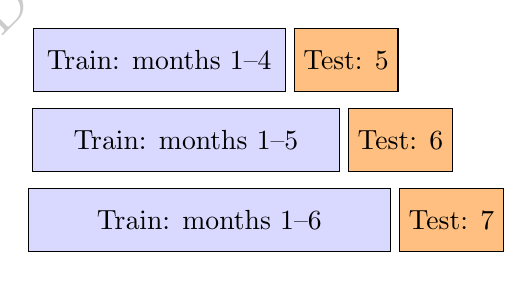
\begin{tikzpicture}[scale=0.85]
        \node[draw,fill=blue!15,minimum width=3.2cm,minimum height=0.8cm] (t1) at (1.6,0) {Train: months 1--4};
        \node[draw,fill=orange!50,minimum width=0.8cm,minimum height=0.8cm,right=1mm of t1] (v1) {Test: 5};

        \node[draw,fill=blue!15,minimum width=3.9cm,minimum height=0.8cm] (t2) at (2.0,-1.2) {Train: months 1--5};
        \node[draw,fill=orange!50,minimum width=0.8cm,minimum height=0.8cm,right=1mm of t2] (v2) {Test: 6};

        \node[draw,fill=blue!15,minimum width=4.6cm,minimum height=0.8cm] (t3) at (2.35,-2.4) {Train: months 1--6};
        \node[draw,fill=orange!50,minimum width=0.8cm,minimum height=0.8cm,right=1mm of t3] (v3) {Test: 7};
    \end{tikzpicture}
\end{lrbox}
\ifdim\wd\bookmeasuredbox<0.65\linewidth
\setlength{\bookcapwidth}{0.65\linewidth}
\else
\setlength{\bookcapwidth}{\wd\bookmeasuredbox}
\fi
\ffigbox[\bookcapwidth]{
\usebox{\bookmeasuredbox}
}{
    \caption{Walk-forward validation across three successive train/test splits.}
    \label{fig:walk_forward}
}
\end{figure}

At each step, the model is refit (or updated) using only data available up to that point, produces a forecast for the next period, and that forecast is scored against the realized outcome once it arrives. The process repeats, rolling forward through the entire sample, and the reported performance is the average across all these genuinely out-of-sample forecasts. This is more computationally expensive than a single train-test split, since the model may be refit many times, but it is the only evaluation procedure that mimics how a forecasting model would actually be used in practice, one period at a time, without ever peeking ahead.

\section{Evaluating Forecast Accuracy}\index{Evaluating Forecast Accuracy}

Once walk-forward validation has produced a sequence of genuinely out-of-sample forecasts, they must be scored using a metric appropriate to the forecasting problem. Beyond the mean squared error used elsewhere in this book, two metrics are especially common in time series work. The root mean squared error (RMSE)\index{Root Mean Squared Error (RMSE)},
\begin{equation*}
\text{RMSE} = \sqrt{\frac{1}{n}\sum_{t=1}^n (\hat X_t - X_t)^2},
\end{equation*}
returns the error to the original units of the series (unlike MSE, which is in squared units), making it directly interpretable, for example, as an average error of ``2.1 basis points'' rather than ``4.4 squared basis points.'' The mean absolute percentage error (MAPE)\index{Mean Absolute Percentage Error (MAPE)},
\begin{equation*}
\text{MAPE} = \frac{100\%}{n}\sum_{t=1}^n \left|\frac{X_t - \hat X_t}{X_t}\right|,
\end{equation*}
expresses errors as a percentage of the actual value, which makes it easier to compare forecast accuracy across series with very different scales (comparing forecast accuracy for a \$10 stock and a \$400 stock in dollar terms is not very meaningful, but a percentage error is). MAPE has a well-known weakness, however: it is undefined when $X_t=0$ and becomes extremely large and unstable when $X_t$ is close to zero, which is a real practical concern for series such as interest rates or spreads that can pass through or near zero, unlike strictly positive prices.

Beyond a single summary statistic, it is standard practice to compare a candidate model's walk-forward RMSE or MAPE against at least one naive benchmark, such as a forecast that simply repeats the last observed value ($\hat X_{t+1} = X_t$) or the simple moving average from Section 7.8. A sophisticated model that cannot outperform this kind of naive benchmark on a walk-forward basis is not adding predictive value, regardless of how compelling its in-sample fit looked, which is exactly the discipline that separates a genuinely useful forecasting model from an elaborate but ultimately unhelpful one.

A small worked comparison shows why this benchmark matters. Suppose a walk-forward evaluation produces five one-step-ahead forecasts for a price series with actual values $100, 102, 98, 105, 101$. A fitted model forecasts $99, 103, 97, 104, 102$, while the naive ``repeat the last value'' benchmark forecasts $98, 100, 102, 98, 105$ (each simply the prior period's actual value). Computing both metrics for each,
\begin{equation*}
\text{RMSE}_{\text{model}} = 1.00, \qquad \text{RMSE}_{\text{naive}} = 4.22, \qquad \text{MAPE}_{\text{model}} = 0.99\%, \qquad \text{MAPE}_{\text{naive}} = 3.73\%,
\end{equation*}
the fitted model beats the naive benchmark by a wide margin on both metrics, roughly a fourfold reduction in RMSE and MAPE alike, giving concrete evidence that the model captures genuine, exploitable structure in the series rather than merely producing forecasts that happen to look reasonable. Had the two RMSE values instead been close, say $4.22$ versus $4.05$, the appropriate conclusion would be the opposite: the model's added complexity is buying almost nothing over simply extrapolating the last observed value, and a practitioner should think hard about whether that complexity is worth the extra estimation risk and maintenance cost.

\section{Challenges in Time Series Forecasting for Finance}

Several challenges recur across almost every time series application in finance.

\textbf{Regime changes and structural breaks.} A model estimated over a calm period, including the AR(1) and GARCH parameters estimated above, can become badly miscalibrated\index{calibration} once the underlying regime shifts, for example when a central bank changes policy or a market enters a crisis. Unlike the smooth, gradual change assumed by a stationary model, a structural break is a sudden shift in the data-generating process itself.

Formal tests exist for detecting a structural break at a known or unknown date (the Chow test and the CUSUM test are two classical examples), but in practice, a combination of periodic re-estimation and the walk-forward validation discipline introduced above is usually a more robust defense than trying to detect every break in real time, since a break severe enough to matter economically is typically also severe enough to show up as a sudden deterioration in walk-forward forecast accuracy.

\textbf{Limited effective sample size.} Financial time series often look large (years of daily data) but contain far less independent information than the raw observation count suggests, because nearby observations are highly correlated. This limits how many parameters can be reliably estimated and is part of why simple, low-order models (AR(1), GARCH(1,1)) so often perform competitively against more elaborate alternatives.

\textbf{Model selection versus overfitting\index{overfitting}.} As in Chapter 6, adding more autoregressive or moving-average terms will always improve the in-sample fit. Coupled with walk-forward validation, information criteria such as AIC and BIC help guard against selecting an overly complex model that fits historical noise rather than a genuine, persistent pattern.

\textbf{Fat tails and non-normality.} Financial returns have more extreme observations than a normal distribution predicts. GARCH models capture time-varying volatility but are often paired with a fatter-tailed error distribution (such as the Student's $t$) to capture this feature, since even a correctly time-varying variance does not by itself guarantee well-calibrated tail forecasts.

\textbf{Multi-step forecasting compounds uncertainty.} A one-step-ahead forecast, like the AR(1) example in this chapter, is usually far more reliable than the same model's five- or twenty-step-ahead forecast, since forecast uncertainty compounds with the horizon. Any decision that depends on a longer-horizon time series forecast should treat that forecast as considerably less certain than a one-step forecast, even when both come from the same fitted model.

\textbf{Spurious cointegration and relationship breakdown.} The pairs-trading strategy in Section~\ref{sec:cointegration} depends on a cointegrating relationship remaining stable, but with enough series to search over, some pairs will appear cointegrated in a historical sample purely by chance, an instance of the same multiple-testing problem raised in Chapter 6. Even a genuine, economically sound cointegrating relationship can break down going forward, for example if a merger, a change in business strategy, or a regulatory shift changes one company's fundamentals relative to its former peer.

\textbf{Model misspecification in multivariate systems.} A VAR model's conclusions, including any Granger-causality test, are sensitive to which variables are included and how many lags are used; omitting a relevant variable that actually drives both series in the system can produce a spurious Granger-causality finding, incorrectly suggesting one included variable predicts another when both are really being driven by the omitted one.

\textbf{Classical models versus neural sequence models.} Every model in this chapter, AR(1), ARIMA, GARCH, and VAR, is a classical statistical model with a small number of interpretable parameters, estimated by OLS or maximum likelihood. A recurrent neural network can, in principle, learn a considerably more flexible mapping from a series' own history to its next value than any fixed linear, fixed-lag-order model this chapter introduced, and Chapter 15 works through exactly such a model, a hand-computed RNN forward pass, in detail.

That added flexibility is not a free upgrade, however: a neural sequence model has many more parameters to fit from data that, as this section's limited-effective-sample-size challenge already noted, contains far less independent information than its raw observation count suggests, so the added flexibility often costs more in overfitting risk than it returns in genuine forecast accuracy unless it is disciplined with exactly the walk-forward validation this chapter introduced.

The practical choice between a classical time series model and a neural sequence model is therefore rarely settled by which is more sophisticated in the abstract, but by which one a limited, noisy financial dataset can actually support without simply memorizing its own history.

\section{A Practical Workflow for Building a Time Series Model}\index{Practical Workflow for Building a Time Series Model}

With this many tools introduced across the chapter, it is useful to close with a single, concrete workflow that ties them together in the order they would typically be applied in practice, summarized in Figure~\ref{fig:ts_workflow}.

\begin{figure}[htbp]
\centering
\begin{lrbox}{\bookmeasuredbox}
    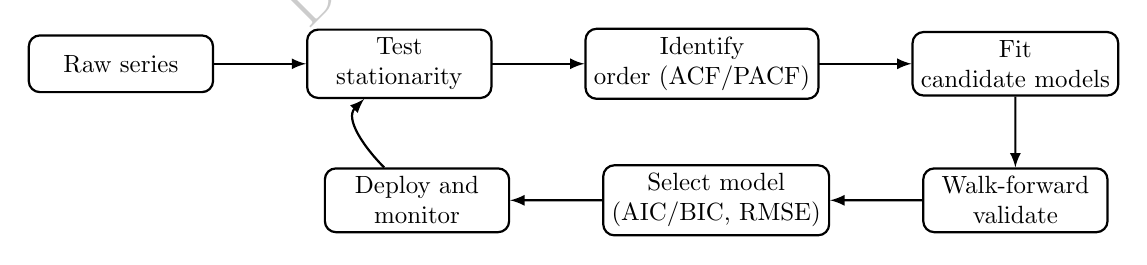
\begin{tikzpicture}[>=latex,thick,node distance=1.3cm,scale=0.9,transform shape]
        \node[draw,rounded corners,minimum width=2.6cm,minimum height=0.8cm,align=center] (raw) {Raw series};
        \node[draw,rounded corners,minimum width=2.6cm,minimum height=0.8cm,right=of raw,align=center] (stationarity) {Test\\stationarity};
        \node[draw,rounded corners,minimum width=2.6cm,minimum height=0.8cm,right=of stationarity,align=center] (identify) {Identify\\order (ACF/PACF)};
        \node[draw,rounded corners,minimum width=2.6cm,minimum height=0.8cm,right=of identify,align=center] (fit) {Fit\\candidate models};
        \node[draw,rounded corners,minimum width=2.6cm,minimum height=0.8cm,below=1.0cm of fit,align=center] (validate) {Walk-forward\\validate};
        \node[draw,rounded corners,minimum width=2.6cm,minimum height=0.8cm,left=of validate,align=center] (select) {Select model\\(AIC/BIC, RMSE)};
        \node[draw,rounded corners,minimum width=2.6cm,minimum height=0.8cm,left=of select,align=center] (monitor) {Deploy and\\monitor};
        \draw[->] (raw) -- (stationarity);
        \draw[->] (stationarity) -- (identify);
        \draw[->] (identify) -- (fit);
        \draw[->] (fit) -- (validate);
        \draw[->] (validate) -- (select);
        \draw[->] (select) -- (monitor);
        \draw[->] (monitor) to[out=135,in=225] (stationarity);
    \end{tikzpicture}
\end{lrbox}
\ifdim\wd\bookmeasuredbox<0.65\linewidth
\setlength{\bookcapwidth}{0.65\linewidth}
\else
\setlength{\bookcapwidth}{\wd\bookmeasuredbox}
\fi
\ffigbox[\bookcapwidth]{
\usebox{\bookmeasuredbox}
}{
    \caption{A practical time series modeling workflow.}
    \label{fig:ts_workflow}
}
\end{figure}

Starting from a raw series, the first step is always to test stationarity (Section~\ref{sec:adf-test}), since every model in this chapter, from AR(1) to GARCH to VAR, assumes some form of stationarity either in levels or after transformation. If the series is non-stationary, difference it (or work with returns, as in Chapter 2) and re-test before proceeding.

Next, the ACF and PACF guide the choice of candidate model orders, following the Box-Jenkins logic introduced in the ARIMA section, rather than guessing arbitrarily or defaulting to the most complex model available. Several candidate specifications are then fit and compared using information criteria (in-sample) and, more importantly, walk-forward validation (out-of-sample), scored with the RMSE or MAPE metrics introduced above and always benchmarked against a naive forecast.

Only once a model has demonstrated genuine walk-forward skill is it deployed, and even then, monitoring continues: the feedback arrow in Figure~\ref{fig:ts_workflow} back to the stationarity test reflects the reality, emphasized throughout this chapter's challenges section, that financial time series are subject to regime changes and structural breaks, so a model that was well-specified last year may need to be re-identified, not just re-fit, as new data arrives.

This workflow applies equally to the single-series models (AR, ARIMA, GARCH) and the multi-series extensions (cointegration testing, VAR) introduced in this chapter; the only difference is that the multivariate case requires checking stationarity and identifying appropriate lag orders for a whole system of series jointly, rather than one series at a time.

\section{Key Takeaways}

Time series methods extend the statistical toolkit of Chapter 6 to data where order matters. Stationarity is the property that makes a fitted model meaningful for the future, and checking for it, formally with the Dickey-Fuller test or informally via the correlogram, is usually the first step in any analysis. The AR(1) example showed how a model's coefficients are estimated by the same OLS logic as any regression, while the GARCH example showed how volatility itself can be modeled and forecast, directly feeding the option pricing and risk models in the chapters that follow.

The cointegration and VAR material extended these ideas from a single series to relationships between series, previewing the pairs-trading strategies of Chapter 11 and the multivariate risk factor models of Chapter 8.

The chapter's closing lesson, walk-forward validation, scored with metrics like RMSE and MAPE and always benchmarked against a naive forecast, is a direct consequence of a single principle repeated throughout this book: a model should never be evaluated using information it would not have had in real time, and it should never be trusted simply because it outperforms a strawman rather than a genuinely competitive baseline.

Several smaller but recurring lessons are worth restating explicitly. The Dickey-Fuller test and the ACF confidence-band calculation both showed, using the chapter's own 8-observation running example, that formal statistical significance is much harder to achieve with small samples than a purely visual reading of a chart or a plausible-looking coefficient might suggest; a quantity that looks convincingly non-zero can still fail to clear a formal significance threshold, and this gap should make an analyst more cautious, not less, about small-sample conclusions.

The comparison between the AR(1) forecast, the simple exponential smoothing forecast, and the Holt's-method forecast for the same series illustrated that different, individually reasonable modeling choices (mean-reversion versus trend extrapolation) can produce meaningfully different point forecasts from identical data, and that choosing between them requires economic judgment about the series' likely future behavior, not just a mechanical best fit to the past.

Finally, the progression from a single series (AR, ARIMA, GARCH) to relationships between series (cointegration, VAR) mirrors a pattern that recurs throughout this book: understanding one object in isolation is usually a prerequisite for, but not a substitute for, understanding how it interacts with the other objects around it, whether those are two cointegrated stock prices here or the many assets in the portfolios of Chapter 10.

\section{Suggested Exercises}

The exercises below span the full range of tools introduced in this chapter, from the basic mechanics of fitting and forecasting a single AR(1) series to testing formally for stationarity, comparing competing forecasting methods, and extending the analysis to relationships between two or more series. Several exercises build directly on the chapter's own worked examples, so your answers can be checked against, or contrasted with, the numbers already computed in the text.

\begin{enumerate}
    \item Explain, in your own words, why fitting an AR(1) model directly to a price series rather than a return series is likely to produce an unreliable model.
    \item Using the data in Table~\ref{tab:ar1_data}, verify by hand that the sample mean is $\bar X = 6.25$ and that $\hat\rho_1 = 0.50$.
    \item Add a ninth observation, $X_9 = 3.0$, to Table~\ref{tab:ar1_data}, refit the AR(1) model, and compare the new $\hat\phi$ and one-step-ahead forecast $\hat X_{10}$ to the values computed in the chapter.
    \item Using the GARCH(1,1) recursion in Table~\ref{tab:garch_recursion}, compute $\sigma_6^2$ if a fifth AssetA return of $r_5 = 0.035$ were observed.
    \item Explain why $\alpha + \beta < 1$ is required for a GARCH(1,1) process to be stationary, and describe what would happen to the variance forecast if $\alpha + \beta = 1$ exactly.
    \item Describe a concrete scenario in which $k$-fold cross-validation, as used in Chapter 6, would give a misleadingly optimistic evaluation of a time series forecasting model.
    \item Discuss one reason a GARCH(1,1) model fit on five years of daily returns during a calm market might forecast volatility poorly at the onset of a financial crisis.
    \item Using the Dickey-Fuller regression in Section~\ref{sec:adf-test}, explain why $\hat\gamma = \hat\phi - 1$, and verify this relationship numerically using the AR(1) coefficient computed in Section~\ref{sec:ar1-example}.
    \item Explain why the Dickey-Fuller test failed to reject the unit-root null hypothesis in Section~\ref{sec:adf-test} even though the fitted AR(1) coefficient clearly indicated mean reversion, and describe what you would expect to happen to the test's conclusion if the same series had 200 observations instead of 8.
    \item Using Table~\ref{tab:pairs_trading}, compute the spread on a hypothetical Day 7 where Stock A trades at 56 and Stock B trades at 51, and explain, using the mean and standard deviation of the historical spread, whether a pairs trader would be more likely to open a new position or close an existing one on that day.
    \item Explain, in your own words, the difference between Granger causality and true causal influence, and describe one financial scenario in which two series could Granger-cause each other without either one truly driving the other.
    \item A retailer's monthly sales data shows a strong, repeating spike every December. Explain why an ordinary ARIMA model without a seasonal component would likely underperform a SARIMA model on this series, and describe what seasonal period $s$ you would use.
    \item Using the multi-step forecasting formulas in Section 7.7, compute the 4-step-ahead AR(1) forecast $\hat X_{12}$ from $X_8=4.0$, and verify it lies between the 3-step and 5-step forecasts already reported in Table~\ref{tab:multistep}.
    \item Using Holt's linear trend method from Section 7.8 with $\alpha=0.5$ and $\beta=0.2$ (instead of $\alpha=0.4$, $\beta=0.3$), recompute the level and trend after processing $X_2=8.0$ through $X_4=7.0$ (three updates starting from $L_1=9.0$, $T_1=-1.0$), and compare your intermediate values to those reported in the chapter.
    \item Using the Kalman filter recursion in Section~\ref{sec:kalman-example}, compute a third update step assuming a new observation $y_3=1.20$ arrives, continuing from $\hat\beta_2\approx 1.132$ and $P_2\approx 0.022$ with the same $Q=0.001$ and $R=0.09$.
    \item Explain, using the workflow in Figure~\ref{fig:ts_workflow}, what step or steps you would need to repeat if a monitoring system detected that a deployed time series model's walk-forward forecast errors had grown substantially larger over the past quarter.
    \item Using the confidence-band rule in Section~\ref{sec:acf-section} ($\pm 1.96/\sqrt{T}$), compute how many observations $T$ would be needed for a sample autocorrelation of $\hat\rho_1=0.50$ to be considered statistically significant at the 95\% level, and comment on how this compares to the 8 observations actually available in Table~\ref{tab:ar1_data}.
    \item Using this chapter's VAR(1) impulse response example, compute $X_1$ and $Y_1$ following a one-unit shock to the exchange rate instead of the interest rate (that is, $X_0=0$, $Y_0=1$), and explain, in terms of the individual coefficients $a_{12}$ and $a_{21}$, why the interest rate's one-period response to an exchange-rate shock turns out to be larger than the exchange rate's one-period response to an interest-rate shock was.
    \item Using this chapter's RMSE/MAPE comparison, recompute both metrics for the naive benchmark if its forecasts were instead $99, 101, 99, 104, 100$ (closer to the actual values than the original naive forecasts), and discuss whether the fitted model would still show a clear advantage over this improved benchmark.
    \item Using Section~\ref{sec:ljung-box}'s Ljung-Box calculation, explain in your own words why a large $Q$ statistic (and correspondingly small $p$-value) is evidence that a model's residuals still contain autocorrelation, and why this counts against the model even though the model's own $R^2$ or fitted coefficients might look reasonable on their own.
    \item Section~\ref{sec:ljung-box} found that AIC and BIC both favor the AR(2) model over the AR(1) model, yet also cautioned that this conclusion may simply reflect overfitting on only six observations. Describe a concrete piece of additional evidence (not just a lower in-sample AIC or BIC) that would make you more confident the AR(2) model is genuinely better specified, not just better fitting.
    \item \textbf{Challenge (real data).} Download at least five years of daily closing prices for a real, liquid stock (for example, via the \texttt{yfinance} library, as Chapter 2 and Chapter 5 already do) and compute its daily log returns. (a) Test the return series for a unit root using the augmented Dickey-Fuller test, as in Section~\ref{sec:adf-test}, and contrast the statistical power of this test on your (likely thousands of) real observations with this chapter's own 8-observation toy example, where the test failed to reject a unit root despite a clearly mean-reverting fitted coefficient. (b) Fit a GARCH(1,1) model to the return series and plot the fitted conditional volatility alongside the raw returns, identifying at least one real historical event (an earnings surprise, a market-wide shock) that produced a visible volatility spike. (c) Compare your fitted $\alpha+\beta$ to the stationarity condition discussed in this chapter, and comment on whether real daily equity returns typically sit close to the $\alpha+\beta=1$ boundary this chapter warns is a sign of near-nonstationary volatility.
\end{enumerate}

\section{Further Reading}

\begin{itemize}
    \item Tsay, \emph{Analysis of Financial Time Series}. Written specifically for financial applications, with extensive coverage of ARIMA, GARCH, and multivariate time series methods including cointegration and VAR models.
    \item Hamilton, \emph{Time Series Analysis}. The classic, mathematically rigorous graduate-level reference for the state-space and Kalman filtering material introduced only briefly in this chapter, alongside a thorough treatment of stationarity and unit-root testing.
    \item Engle, ``Autoregressive Conditional Heteroscedasticity with Estimates of the Variance of United Kingdom Inflation,'' \emph{Econometrica}. The original 1982 paper introducing ARCH models, for readers interested in the primary source behind the GARCH family developed in this chapter.
    \item Hyndman and Athanasopoulos, \emph{Forecasting: Principles and Practice}. A highly practical, freely available online text covering exponential smoothing, ARIMA, and forecast evaluation with an emphasis on applied forecasting workflows like the one in Figure~\ref{fig:ts_workflow}.
    \item Engle and Granger, ``Co-integration and Error Correction: Representation, Estimation, and Testing,'' \emph{Econometrica}. The original paper introducing the cointegration concept and the Engle-Granger two-step testing procedure used in Section~\ref{sec:cointegration}.
    \item Sims, ``Macroeconomics and Reality,'' \emph{Econometrica}. The influential 1980 paper introducing vector autoregression as an alternative to large-scale structural macroeconomic models, foundational to the VAR and Granger-causality material in this chapter.
    \item Litterman and Scheinkman, ``Common Factors Affecting Bond Returns,'' \emph{Journal of Fixed Income}. The original paper documenting the level, slope, and curvature factor structure of the yield curve reproduced in Section~\ref{sec:pca-term-structure}.
\end{itemize}

\end{document}
